\documentclass[12pt,a4paper]{article}
\usepackage[top=25.4mm, bottom=25.4mm, left=19.1mm, right=19.1mm]{geometry}

\usepackage[latin2]{inputenc}
\usepackage{graphicx}
\graphicspath{ {./images/} }
\usepackage{ulem}
\usepackage{amsmath}
\usepackage[document]{ragged2e}

\setlength{\parindent}{4em}
\setlength{\parskip}{1em}
\usepackage{hyperref}

\usepackage{fancyhdr}
\pagestyle{fancy}
\fancyhf{}
\fancyhead[LO]{\textbf{\small IoT and Smart Analytics}\\
\text{\small A Program by IIITH and TalentSprint}}

\usepackage{xcolor}
\usepackage{lipsum}

\rhead{\begin{picture}(0,0) \put(-250,-2){
\includegraphics[width=9cm]{EXP_08_Images/ts-iisc-logo-pr.png}} \end{picture}}
\cfoot{\thepage}


\begin{document}

\begin{center}

\textbf{\large \\EXPERIMENT 23 }\\[6pt]
\text{Making an IoT Cloud and inserting Data to Database using HTTP Post}
\end{center}

\textbf{\large LEARNING OBJECTIVES:}\\[3pt]
At the end of this experiment, participants will be able to:\vspace{-6mm}\begin{enumerate}
 \setlength\itemsep{-0.3em}
\item Understand how sensor data can be stored continuously in a database
\item Create a simple web application \& visualize the live data anywhere in the world
\end{enumerate}

\textbf{\large APPARATUS REQUIRED:}\\
\vspace{-3mm}
\begin{enumerate}
 \setlength\itemsep{-0.3em}
\item ESP32-1pcs 
\item USB cable-1pcs
\item GY-BME280-1pcs
\item Breadboard
\item Internet Connection
\item Jumper Wires
\end{enumerate}

\begin{justify}
\textbf{\large THEORY}\\[3pt]
By performing this experiment, we are going to have our server domain and hosting account where we will store sensor readings from the ESP32. We can visualize/monitor the readings from anywhere in the world by accessing our server domain. Fig.1 below shows the high-level overview of the process involved.\par
\noindent An ESP32 is used as a client that makes an HTTP POST request to a PHP script to insert data (sensor readings) into a MySQL database.\par
\noindent We are going to make a webpage as well that displays the sensor readings, timestamps, and other information from the database.\par 
\noindent As an example, we'll be using a BME280 sensor connected to an ESP32 board. We can modify the code to send readings from a different sensor or use multiple boards. We can also design the webpage as our wish.\par

\noindent Following technology stacks are used in this experiment:
\vspace{-3mm}
\begin{itemize}
\setlength\itemsep{-0.3em}
\item ESP32 programmed with Arduino IDE
\item Free hosting server and domain name
\item PHP \& HTML script to insert data into MySQL and display it on a web page
\item MySQL database to store readings
\end{itemize}


\begin{center} 
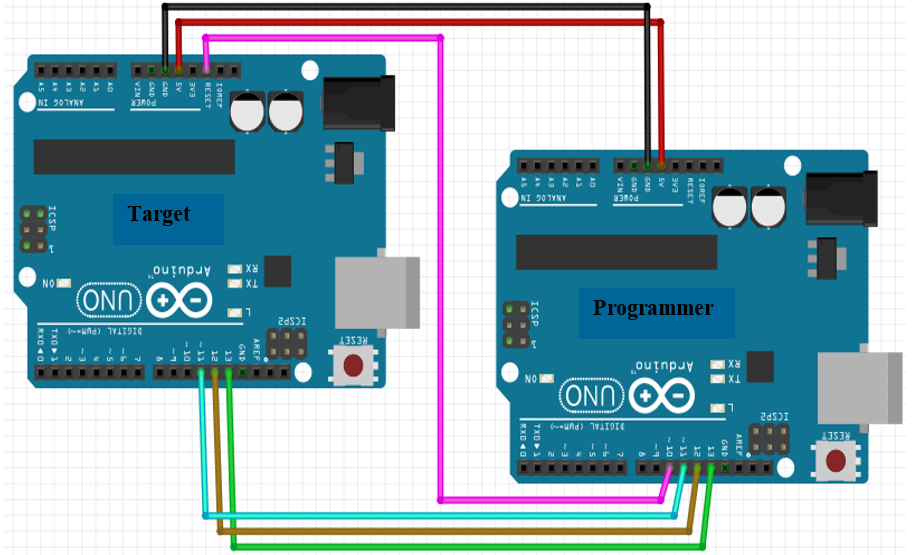
\includegraphics[scale=0.8]{EXP_23_Images/fig1.png}
\end{center}
\begin{center} {Figure 1. Overview of the process involved [1]}\end{center}

\vspace{6pt}
\noindent \textbf{\large PROCEDURE}\\[6pt]
\textbf{A) Getting Hosting and Domain name}\\[3pt]
We will use the free hosting service provided by https://www.000webhost.com/  but any hosting service which supports PHP and MySql will work. Follow the steps below:
\vspace{-3mm}
\begin{enumerate}
\setlength\itemsep{-0.3em}
\item Go to the: https://www.000webhost.com/
\item Choose: Free Web Hosting and click on Free Sign up and make an account\\
You will get an email for confirmation.
\item Login with your credentials and create/provide the name for your website on the control panel.
\end{enumerate}

\noindent \textbf{B) Creating Database}\\[3pt]
We have to create a database where we can store the sensor data that is coming at a certain interval of time continuously. Follow the steps below:
\vspace{-3mm}
\begin{enumerate}
\setlength\itemsep{-0.3em}
\item Go to the Manage Website
\item Toos $ \rightarrow $  DataBase Manager
\item Click on $ \rightarrow $ New Database\\
Provide: Database name, User name, Password\\
You can see DB Name, DB User (with additional id followed by numbers and underscore), and DB Host after a few seconds. Save somewhere this DB Name and DB user and password, these will be used later.
\item Click on Manage and go to PhpMyAdmin
\item Select the database by clicking  the database name on the left side
\item Choose the SQL tab and paste the query below and click on Go.
\end{enumerate}

\fbox{\begin{minipage}{40em}
\noindent {CREATE TABLE SensorData (\\
id  INT(6)  UNSIGNED AUTO\_INCREMENT PRIMARY KEY,\\
sensor  VARCHAR(30)  NOT  NULL,\\
reading\_time TIMESTAMP  DEFAULT  CURRENT\_TIMESTAMP \\
ON  UPDATE CURRENT\_TIMESTAMP,\\
location  VARCHAR(30)  NOT  NULL, \\
Temp  VARCHAR(10), \\
Humi  VARCHAR(10), \\
Pres  VARCHAR(10)\\
) \\}
\end{minipage}}




\noindent \textbf{C) Creating web application}\\[3pt]
Now we have to develop two PHP scripts, one for inserting data into MySQL Database and another for displaying the content of the database on the webpage. A zip file named 'script' has been provided which contains all the code files needed for this experiment. Unzip the file and save two PHP scripts and one Arduino script. Follow the steps below:
\vspace{-3mm}
\begin{enumerate}
\setlength\itemsep{-0.3em}
\item Tools $ \rightarrow $ File Manager $ \rightarrow $ Upload files
\item Go inside public\_html\\
You can see different options upon hovering the cursor over the toolbar. Click on the new folder and name it as 'API'.

\item Inside API folder $ \rightarrow $ Upload the following file:\\
$ \rightarrow $ esp-data.php\\
$ \rightarrow $ post-esp-data.php

These files can be opened/edited with Notepad. Don't forget to change the DB Name, DB User, and Password according to your setting.
\end{enumerate}

\noindent \textbf{D)	Sensor integration \& ESP32 firmware}\\[3pt]
Now BME280 sensor is connected with ESP32. There are several versions of this sensor module. The BME280 sensor uses I2C or SPI communication protocol to exchange data with a microcontroller. Pin configuration for six/four-pin versions is given in the table below. The Six-pin version may operate in both I2C and SPI communication protocols. While using BME280 with I2C communication SCK pin acts as SCL and SDI pin acts as SDA pin and leaves SDO and CS pin unconnected.

\vspace{8cm}

\begin{center} {Table 1. Pin configuration for integration of  BME 280 \& ESP32}\end{center}
\vspace{-8mm}
\begin{center} 
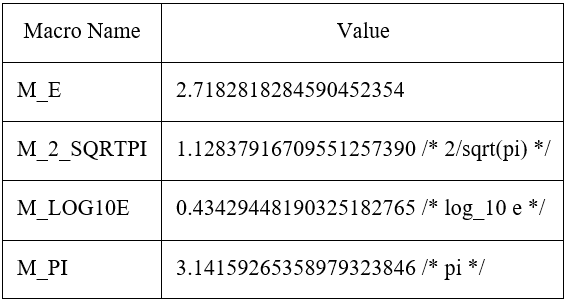
\includegraphics[scale=0.7]{EXP_23_Images/table1.png}
\end{center}
 \noindent After completing the connection as given in the table above, we need to upload the firmware named 'esp\_sql\_php.ino' from PC to ESP32. Don't forget to change the network credentials (ssid \& password). Completing all the above steps, write your domain name followed by '/esp-data.php' for eg. https://rameniot.000webhostapp.com/esp-data.php in your browser and you can see the live data table.

\vspace{10pt}
\noindent \textbf{\large REFERENCES:}
\vspace{-6mm}
\begin{enumerate}
\setlength\itemsep{-0.3em}
\item  \href {https://randomnerdtutorials.com/esp32-esp8266-mysql-database-php}{Insert Data into MySQL Database using PHP and Arduino IDE}

\end{enumerate}
\end{justify}
\end{document}